\section{AWS Lambda}\label{chapter:aws_lambda}

AWS Lambda to konkretna implementacja funkcji jako usługi oferowana przez Amazon Web Services od 2015 roku.
W ramach rozdziału opisano działanie usługi, wraz z jej najważniejszymi z perspektywy programisty cechami.
Skupiono się na konkretnym użyciu języka Java, który jest dostępny w serwisie.

AWS Lambda była pierwszą platformą FaaS oferowaną przez dużego dostawcę chmurowego.
Znacząco przyczyniło się to do popularyzacji paradygmatu bezserwerowego.
Usługa ta implementuje założenia modelu funkcji jako usługi, oferując programistom możliwość uruchamiania kodu bez konieczności zarządzania infrasktrukturą.
AWS Lambda przejmuje odpowiedzialność za przydzielenie zasobów, skalowanie, monitorowanie oraz zarządzanie cyklem życia wykonywanych funkcji.
Umożliwia to twórcom oprogramowania skupienie się na logice biznesowej aplikacji, rozliczając ich jedynie za faktyczny czas obliczeń i liczbę wywołań.

\begin{figure}[h]
    \centering
    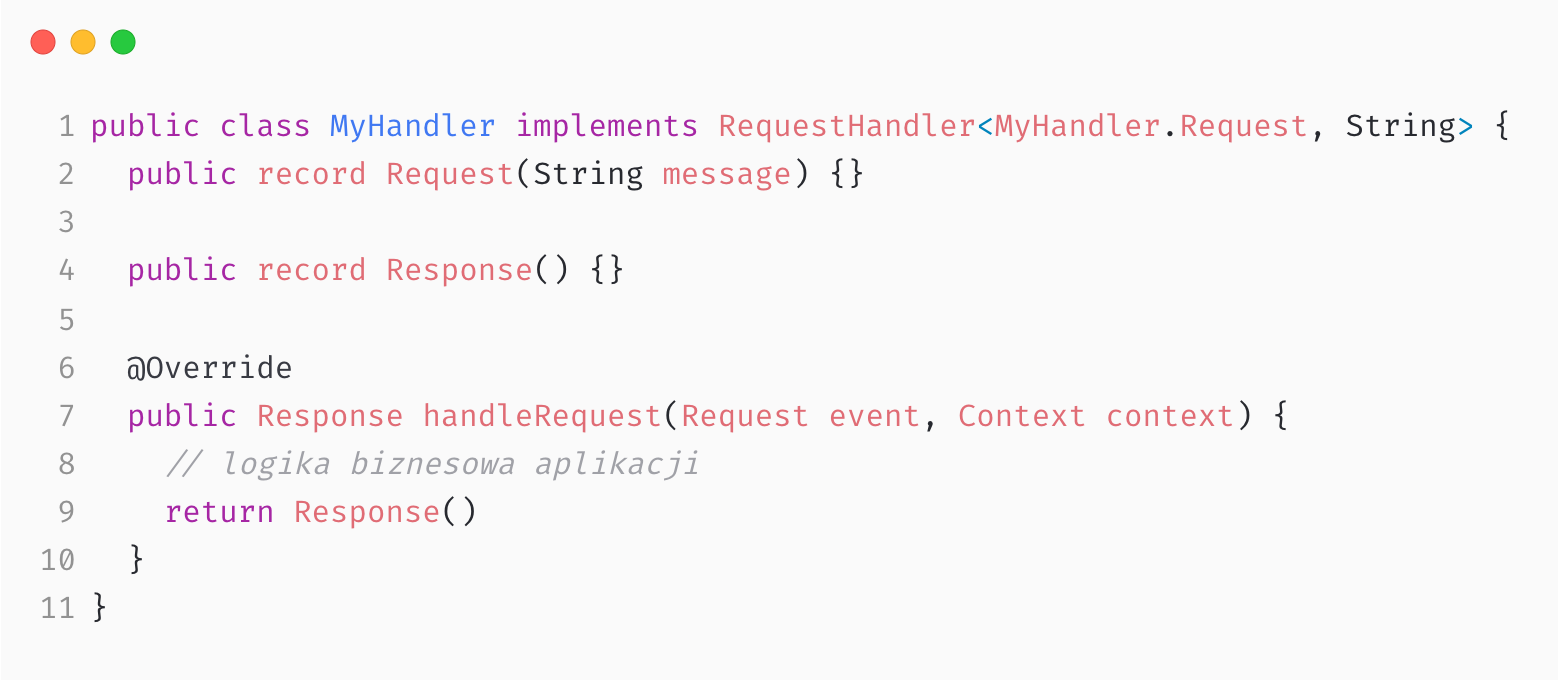
\includegraphics[width=0.95\textwidth]{charts/sample-lambda-code.png}
    \caption{Przykładowa implementacja funkcji AWS Lambda w języku Java [źródło: opracowanie własne]}
    \label{fig:example_aws_lambda}
\end{figure}

Pierwszym krokiem wdrożenia funkcji AWS Lambda jest napisanie uruchamianego kodu.
Przykładowa implementacja została przedstawiona na Rysunku \ref{fig:example_aws_lambda}. 
Odpowiedni interfejs, który wykorzystuje programista, jest dostarczany przez AWS.
Jego implementacja w klasie MyHandler pozwala na nadpisanie metody handleRequest, która jest wywoływana w momencie obsługi zdarzenia.
W ciele metody umieszczana jest konkretna logika biznesowa funkcji chmurowej, na której skupia się użytkownik.

Aby kod został uruchomiony w chmurze należy utworzyć nową funkcję AWS Lambda.
Może to być wykonane poprzez konsolę Amazon Web Services, AWS CLI (ang. Command Line Interface) lub narzędzia infrasktruktury jako kod (np. AWS CDK, Terraform) \cite{awsLambdaDocs}.
Niezbędne do tego jest przygotowanie zasobów do wdrożenia.
Może to być wykonane na dwa sposoby: poprzez pliki ZIP lub JAR (istnieje także możliwość wdrożenia obrazów Dockerowych, jednak w ramach podrozdziału skupiamy się na środowisku uruchomieniowym Java) \cite{awsLambdaDocs}.
Tak przygotowany plik jest gotowy do wdrożenia podczas uruchamiania funkcji.

Kolejnym krokiem jest skonfigurowanie funkcji w usłudze AWS Lambda, co obejmuje zdefiniowanie kluczowych parametrów \cite{awsLambdaDocs}.
Jednym z najważniejszych jest pamięć funkcji, która odpowiada ilości pamięci RAM w megabajtach.
Innym parametrem jest limit czasu wykonania, który definiuje maksymalny czas, przez jaki pojedyncze wywołanie funkcji może być przetwarzane, zanim zostanie automatycznie zakończone przez platformę. 
Dodatkowo, programista ma możliwość zdefiniowania zmiennych środowiskowych, które pozwalają na przekazywanie konfiguracji do kodu funkcji w czasie jej działania.

Aby funkcja mogła zostać zintegrowana z tworzonym systemem należy skonfigurować źródła zdarzeń.
Zgodnie z naturą FaaS, funkcje Lambda są projektowane do uruchamiania w odpowiedzi na zdarzenia pochodzące z szerokiego ekosystemu usług AWS lub źródeł zewnętrznych.
Do typowych usług integrujących się z Lambda jako wyzwalacze należą m.in. \cite{awsLambdaDocs}:
\begin{itemize}
    \item Amazon S3 (np. przy tworzeniu nowego obiektu),
    \item Amazon API Gateway (dla żądań HTTP),
    \item Amazon DynamoDB Streams (reakcja na zmiany w tabelach),
    \item Amazon SQS (nowe wiadomości w kolejce),
    \item Amazon SNS (powiadomienia tematyczne),
    \item Amazon EventBridge (dla zdarzeń harmonogramowych oraz zdarzeń z innych usług i aplikacji).
\end{itemize}
Dzięki temu programista określa, w jakich okolicznościach i z jakimi danymi wejściowymi funkcja Lambda ma zostać automatycznie uruchomiona.
Poprzez skonfigurowane wcześniej zdarzenia funkcja może zostać uruchomiona, co zachodzi w ramach określonego cyklu życia.
Składa się on z trzech etapów: inicjalizacji, wywołania i wyłączenia \cite{awsLambdaDocs}, przedstawionych na Rysunku \ref{fig:aws_lambda_lifecycle}.

\begin{figure}[h]
    \centering
    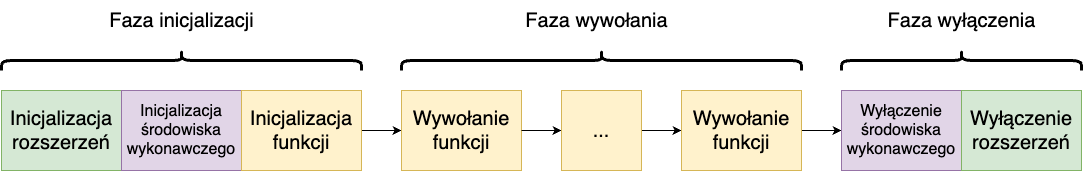
\includegraphics[width=0.95\textwidth]{charts/aws_lambda_lifecycle.drawio.png}
    \caption{Cykl życia funkcji AWS Lambda [źródło: opracowanie własne na bazie dokumentacji AWS Lambda \cite{awsLambdaDocs}]}
    \label{fig:aws_lambda_lifecycle}    
\end{figure}

Pierwszym etapem uruchomienia funkcji jest faza inicjalizacji, która wykonuje się gdy zasoby nie są jeszcze przydzielone.
Składa się ona z trzech mniejszych etapów \cite{awsLambdaDocs}: 
\begin{itemize}
    \item Inicjalizacji rozszerzeń (np. narzędzia do monitorowania)
    \item Inicjalizacji środowiska wykonawczego (np. maszyny wirtualnej Java)
    \item Inicjalizacji funkcji (uruchomienie kodu statycznego funkcji)
\end{itemize}

Po fazie inicjalizacji, gdy środowisko wykonawcze jest już przygotowane, następuje właściwa faza wywołania funkcji.
Rozpoczyna się ona, gdy platforma Lambda przesyła zdarzenie do przygotowanego środowiska uruchomieniowego.
W ten sposób inicjowane jest wykonanie kodu funkcji. 
Całkowity czas trwania tej fazy jest ściśle ograniczony przez skonfigurowany wcześniej limit czasu wykonania. 
Faza wywołania kończy się, gdy środowisko uruchomieniowe zakończy swoje zadania i zasygnalizuje gotowość do obsługi kolejnego żądania poprzez wysłanie komunikatu do usługi Lambda.

Ostatnim etapem w cyklu życia środowiska wykonawczego AWS Lambda jest faza wyłączenia.
Następuje on gdy usługa decyduje o zakończeniu działania konkretnego środowiska uruchomieniowego (np. z powodu zmniejszenia aktywności).
Po tej fazie zasoby dostawcy chmurowego zostają zwolnione.

Istotne dla działania AWS Lambda są tak zwane zimne i ciepłe starty, które wynikają bezpośrednio z cyklu życia funkcji.
Aby umożliwić wywołanie, platforma AWS Lambda musi pobrać kod użytkownika, a następnie utworzyć nowe środowiska wykonawcze.
Fazy te są określane jako tzw. zimne starty (ang. cold starts) \cite{awsLambdaDocs}, co zostało przedstawione na Rysunku \ref{fig:aws_lambda_warm_cold_starts}.
Dostawca chmurowy nie pobiera opłaty za czas trwania tych etapów, jednak wpływają one na ogólną wydajność funkcji.
Po przygotowaniu środowiska może zostać uruchomiony kod (inicjujący oraz obsługujący funkcje).
Następnie, środowisko wykonawcze funkcji jest zatrzymywane, jednak nie usuwane.
Pozwala to następnie na jego ponowne użycie (przez pewien określony czas), co pozwala na szybsze uruchomienie funkcji.
Zjawisko to nazywane jest ciepłym startem (ang. warm start) \cite{awsLambdaDocs}.

\begin{figure}[h]
    \centering
    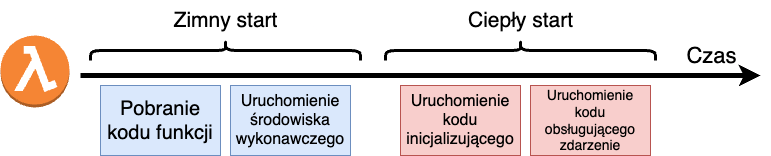
\includegraphics[width=0.95\textwidth]{charts/warm_cold_starts_lambda.png}
    \caption{Proces uruchomienia AWS Lambda w kontekście zimnych i ciepłych startów [źródło: opracowanie własne na bazie dokumentacji AWS Lambda \cite{awsLambdaDocs}]}
    \label{fig:aws_lambda_warm_cold_starts}    
\end{figure}

% \begin{lstlisting}[
%     caption={Przykładowa implementacja funkcji AWS Lambda w języku Java [źródło: opracowanie własne]}, 
%     label={code:example_aws_lambda},
% ]
% public class MyHandler implements 
%     RequestHandler<MyHandler.Request, String> {
    
%     public record Request(String message) {}

%     public record Response() {}

%     @Override
%     public Response handleRequest(Request event, Context context) {
%         // logika biznesowa funkcji
%         return Response()
%     }
% }
% \end{lstlisting}
